% Template for ICIP-2019 paper; to be used with:
%          spconf.sty  - ICASSP/ICIP LaTeX style file, and
%          IEEEbib.bst - IEEE bibliography style file.
% --------------------------------------------------------------------------
\documentclass{article}
\usepackage{spconf,amsmath,graphicx, cite}

% Example definitions.
% --------------------
\def\x{{\mathbf x}}
\def\L{{\cal L}}

% Title.
% ------
\title{Computer Security Report}
%
% Single address.
% ---------------
\name{Junsong Yang}
\address{School of Computer Science \\ University of Nottingham}
%
% For example:
% ------------
%\address{School\\
%	Department\\
%	Address}
%
% Two addresses (uncomment and modify for two-address case).
% ----------------------------------------------------------
%\twoauthors
%  {A. Author-one, B. Author-two\sthanks{Thanks to XYZ agency for funding.}}
%	{School A-B\\
%	Department A-B\\
%	Address A-B}
%  {C. Author-three, D. Author-four\sthanks{The fourth author performed the work
%	while at ...}}
%	{School C-D\\
%	Department C-D\\
%	Address C-D}
%
\begin{document}
%\ninept
%
\maketitle
%

\section{Passwords}
\label{sec:passwd}

In this section, the designed password and authentication policy will be proposed and justified.
First, the password policy will be explained in detail with additional authentication measures.
Then, mechanisms of storing passwords will be entailed.

\subsection{Password Policy}
The design of the policy is the result of balancing complexity and overall security. 
As Gollmann \cite{GollmannDieter2011Cs/D}suggested, the overall security may be diminished 
if one security mechanism is overstated. Users tend to bypass the mechanism if it is too 
inappropriate for them to properly work with, hence the overall security of the system 
may be weakened. By considering that, the following password policies are proposed.

\subsubsection{Password Length}
This policy enforces the minimum number of character required to use as a valid password. 
Generally, the short the password, the more like and easily to be cracked by brute-forcing.
Hence, by setting the minimum password length to ten, the difficulty for brute-forcing password 
cracking would be noticeably increased.

\subsubsection{Password Format}
This policy intended to accumulating the strength of the valid password by requiring what and 
how many kinds of character must be included in a password. By requiring the password to contain 
at least one lower and upper letter, one number, and one special character, combining with 
password length policy, the possibility of successful brute-force cracking would significantly decreasing.

\subsubsection{Password Ageing}
This policy requires users to change their password periodically. The likelihood of password 
breaching would increase as time goes by, hence this is a appropriate approach to eliminate the 
risk of potential breaching.

\subsubsection{Password Use}
To further diminishing the risk of potential password breaching over time, additional mechanism 
need to be employed to block users from using the same password twice. This policy is essential 
to assist the password ageing policy to fulfil its purpose.


\subsubsection{Login Attempts}

\subsection{Additional Authentication Measures}

TOCTTOU and Biometrics

\subsection{Storing Passwords}

\section{Firewalls}
\label{sec:firewalls}

%%%%%%%%%%%%%%%%%%% NOTES %%%%%%%%%%%%%%%%%%%%%%%%

%%%%%%%%%%%%%%%%%%% NOTES %%%%%%%%%%%%%%%%%%%%%%%%

\section{Server Security}
\label{sec:serversec}

%%%%%%%%%%%%%%%%%%% NOTES %%%%%%%%%%%%%%%%%%%%%%%%

%%%%%%%%%%%%%%%%%%% NOTES %%%%%%%%%%%%%%%%%%%%%%%%


% Below is an example of how to insert images. Delete the ``\vspace'' line,
% uncomment the preceding line ``\centerline...'' and replace ``imageX.ps''
% with a suitable PostScript file name.
% -------------------------------------------------------------------------
\begin{figure}[htb]

\begin{minipage}[b]{1.0\linewidth}
  \centering
  \centerline{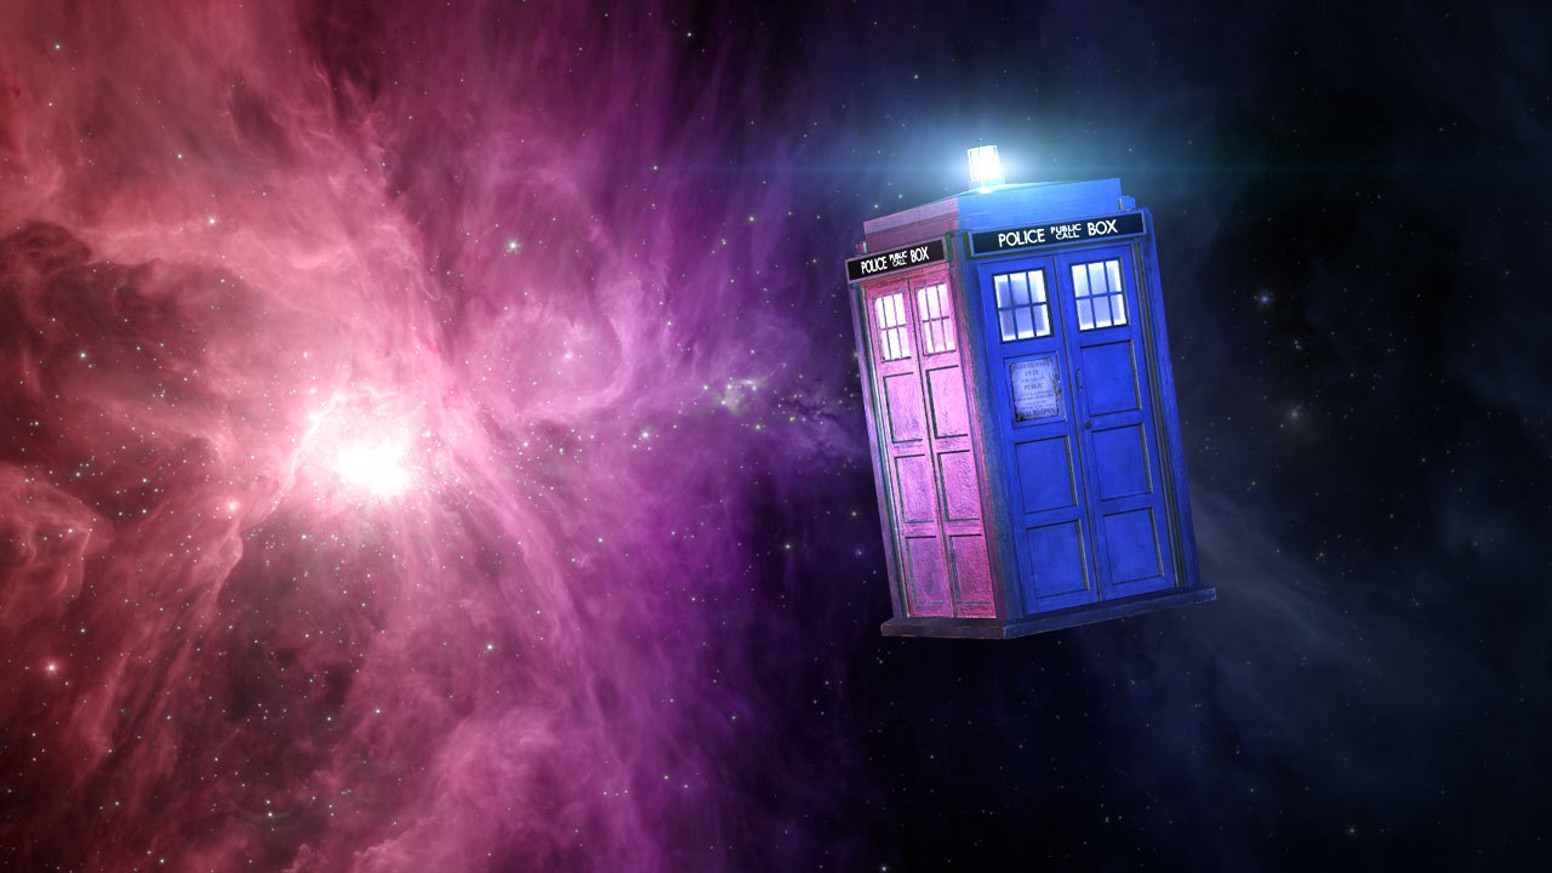
\includegraphics[width=8.5cm]{image1}}
%  \vspace{2.0cm}
  \centerline{(a) Result 1}\medskip
\end{minipage}
%
\begin{minipage}[b]{.48\linewidth}
  \centering
  \centerline{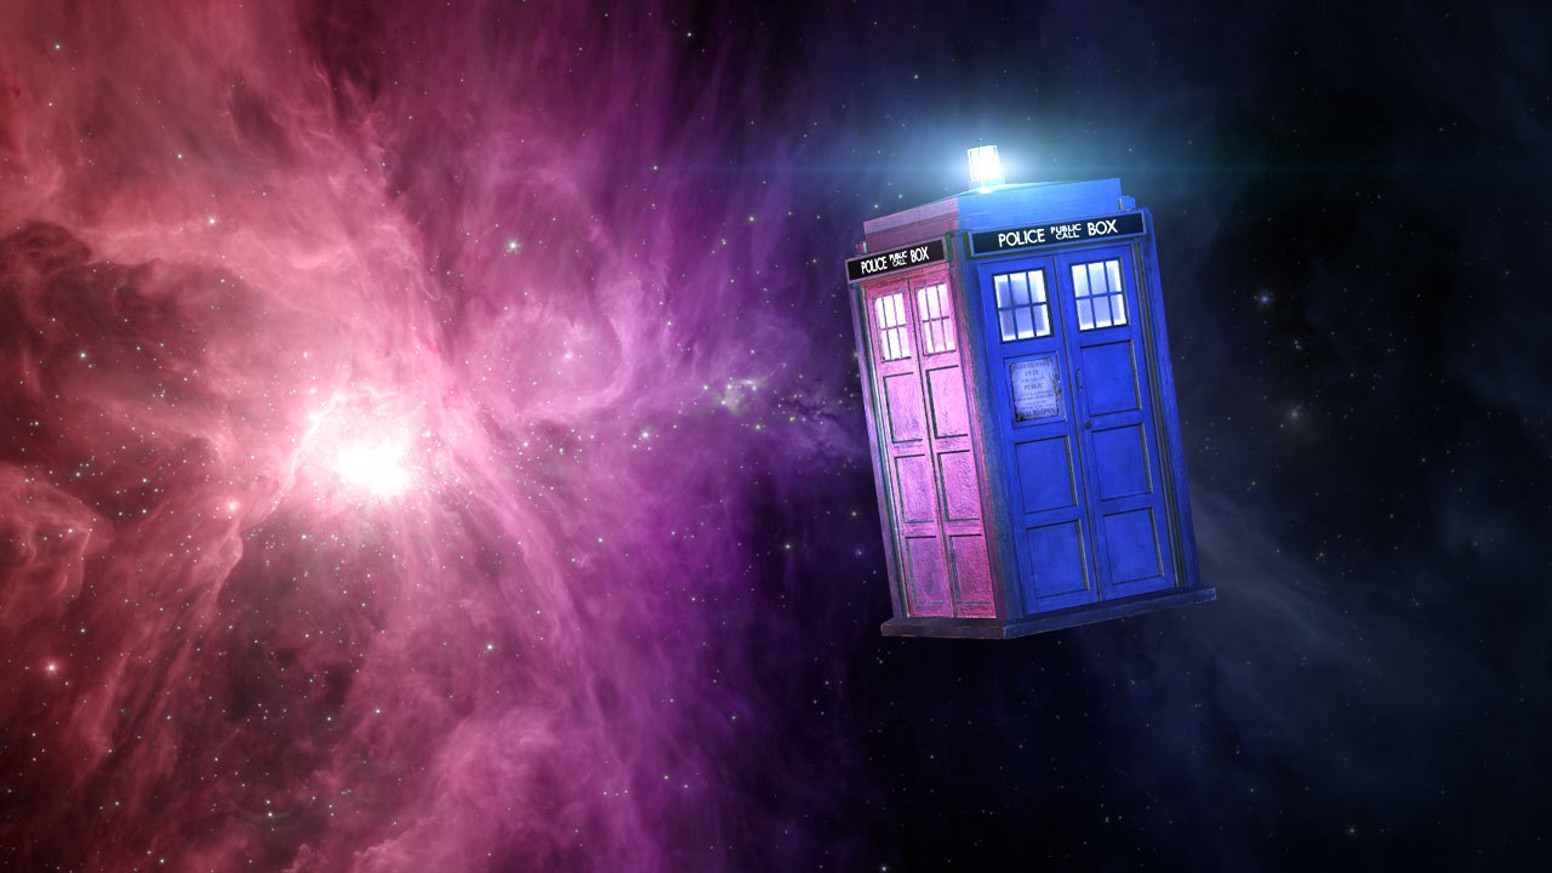
\includegraphics[width=4.0cm]{image1}}
%  \vspace{1.5cm}
  \centerline{(b) Results 3}\medskip
\end{minipage}
\hfill
\begin{minipage}[b]{0.48\linewidth}
  \centering
  \centerline{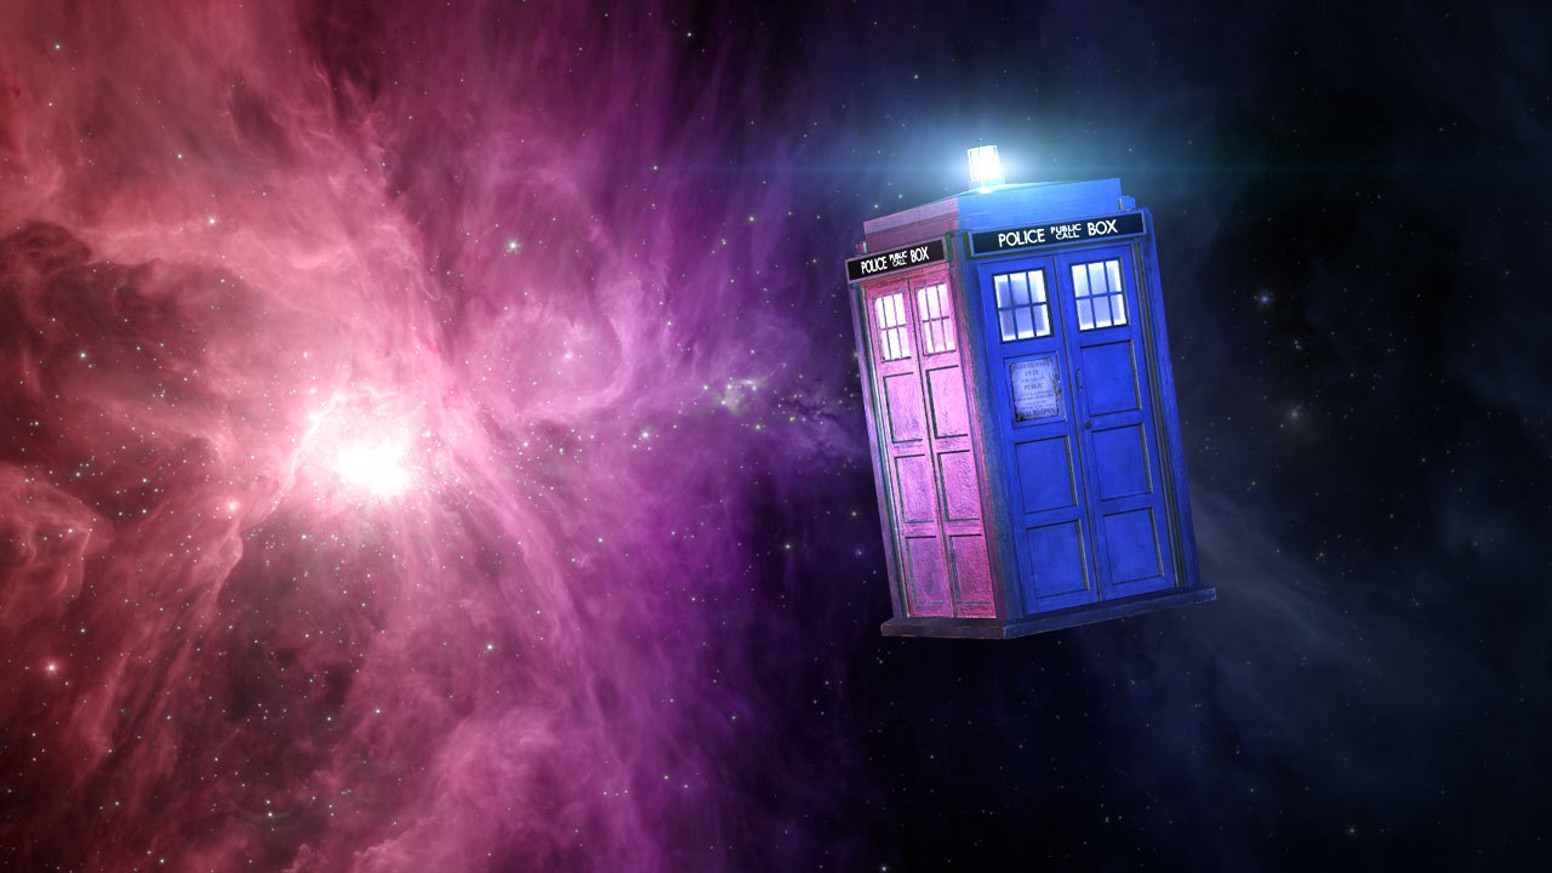
\includegraphics[width=4.0cm]{image1}}
%  \vspace{1.5cm}
  \centerline{(c) Result 4}\medskip
\end{minipage}
%
\caption{Example of placing a figure with experimental results.}
\label{fig:res}
%
\end{figure}


% To start a new column (but not a new page) and help balance the last-page
% column length use \vfill\pagebreak.
% -------------------------------------------------------------------------
%\vfill
%\pagebreak

\bibliographystyle{IEEEbib}
\bibliography{bibtex}

\end{document}
